% ============================================================
%  StudyVault – BCA Project Report
%  Author  : Bineeth Baby
%  Reg. No : 230021085633
%  College : St. George's College Aruvithura
%  Univ.   : Mahatma Gandhi University
% ============================================================
\documentclass{sgcproject}

% ---- Essential packages ------------------------------------
\usepackage{graphicx}       % \includegraphics
\usepackage{float}          % [H] figure placement
\usepackage{booktabs}       % professional table rules
\usepackage{array}          % p{} column type
\usepackage{url}            % \url{}
\usepackage{appendix}       % \begin{appendices}
\usepackage{listings}       % code listings
\usepackage{xcolor}         % colour in listings
\usepackage{microtype}      % better text justification

% ---- Code listing style ------------------------------------
\lstset{
  basicstyle=\small\ttfamily,
  breaklines=true,
  breakatwhitespace=true,
  keywordstyle=\bfseries\color{blue!70!black},
  commentstyle=\itshape\color{gray},
  stringstyle=\color{orange!80!black},
  showstringspaces=false,
  frame=single,
  numbers=left,
  numberstyle=\tiny\color{gray},
  numbersep=5pt,
  xleftmargin=1.5em,
  framexleftmargin=1.5em,
  tabsize=4,
}

% ---- Graphics search path ----------------------------------
%  All images live in report/images/ (same folder as report.tex)
\graphicspath{{images/}}

% ---- Float spacing (compact, matches university style) ------
\setlength{\textfloatsep}{10pt}   % space between float and text
\setlength{\floatsep}{8pt}        % space between two floats


% ---- Document metadata -------------------------------------
\title{StudyVault -- Online Notes Sharing Platform with AI Moderation}
\author{Bineeth Baby}
\regno{230021085633}

% ============================================================
\begin{document}
% ============================================================

\maketitle
\makecert

% ============================================================
%  ABSTRACT
% ============================================================
\newpage
\pagenumbering{roman}
\setcounter{page}{1}
\newgeometry{top=4cm,bottom=0.1cm}
\renewcommand\abstractname{ABSTRACT}
\begin{abstract}
\vspace{5cm}

StudyVault is a centralised, role-based academic notes sharing platform developed for educational institutions affiliated to Mahatma Gandhi University. The platform enables students to upload study notes that are automatically screened by an Artificial Intelligence (AI) safety engine before being reviewed and approved by faculty members. Only faculty-approved notes are made available to the broader student community, ensuring academic quality and content integrity.

The system supports three distinct user roles---Student, Faculty, and Administrator---each with a dedicated dashboard, access controls, and workflow. Core features include multi-file upload with drag-and-drop support, AI-powered content safety analysis using Groq's Llama~3.1-8B-Instant model, a faculty approval workflow (Approve\,/\,Reject\,/\,Return), browse and download of approved notes, a favourites library, a real-time notification system, private messaging, a community discussion forum, AI study assistant tools (summariser, flashcard generator, Q\&A bot, and study guide generator), and a comprehensive administrator dashboard with analytics, moderation controls, and system configuration.

The backend is built with \textbf{FastAPI} (Python), the database layer uses \textbf{MongoDB}, the frontend is rendered with \textbf{Jinja2} templates, and AI capabilities are provided by the \textbf{Groq API}. The system was tested across all three roles and all major user workflows, with all test cases passing successfully.

\end{abstract}

% ============================================================
%  ACKNOWLEDGMENT
% ============================================================
\newpage
\chapter*{ACKNOWLEDGMENT}
\addcontentsline{toc}{chapter}{ACKNOWLEDGMENT}

I present this report describing the main project completed during the sixth semester of the BCA course. I express my sincere gratitude to my Project Coordinator, \textbf{Dr. Jestin Joy}, Head of the Department of Computer Applications, for his constant guidance, encouragement, and valuable suggestions throughout the development of this project.

I extend my heartfelt thanks to my Project Guide, \textbf{Dr. Soumya George}, Assistant Professor, Department of Computer Applications, for her continuous support, timely advice, and expert guidance which played a significant role in the successful completion of this project.

I also express my sincere appreciation to \textbf{Dr. Gemini George}, \textbf{Dr. Anu Thomas}, and \textbf{Mr. Linu T. James} for their valuable support and encouragement during the course of this work. I also thank our Principal, \textbf{Prof. Dr. Siby Joseph}, for providing the academic environment and facilities necessary for completing this project.

Finally, I thank my parents, family members, friends, and well-wishers for their constant support, motivation, and encouragement throughout the development of this project.

\begin{flushright}
\textbf{Bineeth Baby}
\end{flushright}

% ============================================================
%  FRONT MATTER
% ============================================================
\newpage
\restoregeometry
\tableofcontents
\newpage

\cleardoublepage
\addcontentsline{toc}{chapter}{\listfigurename}
\listoffigures
\newpage

\cleardoublepage
\addcontentsline{toc}{chapter}{\listtablename}
\listoftables
\newpage

\pagestyle{plain}

% ============================================================
%  CHAPTER 1 – INTRODUCTION
% ============================================================
\chapter{INTRODUCTION}
\pagenumbering{arabic}
\setcounter{page}{1}
\renewcommand{\baselinestretch}{1.50}

\section{Overview}

The rapid expansion of digital education has fundamentally changed how students interact with academic content. Traditional approaches to sharing study material---photocopies, WhatsApp forwards, and scattered email attachments---lack structure, accountability, and quality control. In academic institutions where subjects span multiple semesters and faculty oversee large student groups, there is a growing need for a centralised, organised, and verifiable system for distributing study notes.

The proliferation of smartphones and internet access has made it practical to build such platforms as web applications, accessible from any device with a browser. However, most available platforms are generic file-sharing tools that do not account for academic-specific needs such as faculty review, role-based access, or the monitoring of content quality. This gap motivates the development of a purpose-built academic notes sharing system.

StudyVault was conceived to fill this gap by providing a structured digital environment where students can upload their study notes, faculty can review and approve them, and administrators can maintain oversight of the entire platform---all in one cohesive web application.

\section{Problem Statement}

Students in academic institutions face several recurring problems with access to quality study material:

\begin{itemize}
    \item Notes are shared through informal channels with no quality verification.
    \item There is no mechanism to ensure that shared content is accurate, appropriate, or academically sound.
    \item Faculty have no oversight of student-generated content being circulated among peers.
    \item Students who miss classes have no reliable platform to access peer-reviewed notes.
    \item AI-generated or plagiarised content can easily be passed off as original notes.
\end{itemize}

These problems result in the distribution of unreliable, low-quality, or even inappropriate academic content, ultimately harming the educational process.

\section{Need for the Proposed System}

StudyVault addresses the above problems by introducing a structured, role-based workflow for academic notes sharing. The need for such a system is clear:

\begin{itemize}
    \item \textbf{Quality Assurance:} Only faculty-approved notes are made publicly accessible to students.
    \item \textbf{AI Safety Screening:} Every uploaded note is automatically analysed by an AI model for plagiarism, inappropriate content, spam, and academic misconduct before human review begins.
    \item \textbf{Role Separation:} Students, faculty, and administrators each have clearly defined access rights and responsibilities.
    \item \textbf{Centralised Access:} All approved notes are browsable and downloadable from a single platform.
    \item \textbf{Communication and Community:} Built-in messaging, a discussion forum, and notifications keep all users connected.
\end{itemize}

\section{Objectives of the Project}

The objectives of StudyVault are:

\begin{enumerate}
    \item To build a secure, role-based web platform on which students can upload study notes and faculty can review and publish them.
    \item To integrate AI-driven content analysis (using the Groq API with Llama 3.1-8B) to automatically flag inappropriate, plagiarised, or low-quality content before faculty review.
    \item To implement a session-based authentication system that enforces strict role separation between students, faculty, and administrators.
    \item To provide a notification system that keeps all users informed about the status of their notes, messages, and system events in real time.
    \item To build a discussion forum and private messaging system to support academic collaboration.
    \item To give administrators complete oversight of users, notes, reports, announcements, and system configuration from a single admin dashboard.
\end{enumerate}

\section{Scope of the System}

StudyVault is scoped as a single-institution academic notes platform. The system covers:

\begin{itemize}
    \item \textbf{User Management:} Registration and login for three roles---Student, Faculty, and Admin.
    \item \textbf{Notes Lifecycle:} Upload, AI safety check, faculty review (Approve\,/\,Reject\,/\,Return), publication, browsing, and download.
    \item \textbf{Communication:} Private messaging between all users, a faculty-to-student announcement system, and a community discussion forum.
    \item \textbf{AI Tools:} AI summary generation, flashcard creation, Q\&A answers, and study guide generation for students via the Groq API.
    \item \textbf{Administrative Control:} User activation/deactivation, content moderation, platform settings configuration, and report management.
\end{itemize}

The system does not currently include real-time chat (WebSocket), video content, or integration with external Learning Management Systems (LMS).

\section{Major Features of the System}

\begin{table}[H]
\centering
\begin{tabular}{|p{4cm}|p{10cm}|}
\hline
\textbf{Feature} & \textbf{Description} \\
\hline
Role-Based Login & Separate portals for Student, Faculty, and Admin with role-enforced session checks \\
\hline
Notes Upload & Multi-file upload with drag-and-drop support; subject and title tagging \\
\hline
AI Safety Analysis & Automatic content scanning using Groq Llama~3.1-8B for 6 violation categories \\
\hline
Faculty Review Workflow & Notes can be Approved, Rejected, or Returned with feedback \\
\hline
Browse and Download & Approved notes are searchable and downloadable by all students \\
\hline
Favourites & Students can save and manage a personal library of notes \\
\hline
Notifications & Real-time badge-count notifications for all events \\
\hline
Private Messaging & Direct messaging between students, faculty, and admins \\
\hline
Discussion Forum & Community Q\&A board with thread support \\
\hline
AI Study Tools & Summariser, Flashcard Generator, Q\&A Bot, and Study Guide Generator \\
\hline
Admin Dashboard & Analytics, faculty performance, moderation queue, and system settings \\
\hline
Content Reporting & Students or faculty can report notes; admin resolves reports \\
\hline
\end{tabular}
\caption{Major Features of StudyVault}
\end{table}

% ============================================================
%  CHAPTER 2 – RELATED WORK
% ============================================================
\chapter{RELATED WORK}

\section{Overview of Existing Systems}

Several platforms exist that partially address the need for academic notes sharing. A review of three major systems is presented below.

\subsection{Google Drive / Google Classroom}

Google Drive allows users to upload and share files with others via shared folders. Google Classroom adds a layer of organisation by letting teachers create ``classrooms'' and post resources. However, both are general-purpose tools not specifically designed for academic notes management.

\textbf{Limitations:}
\begin{itemize}
    \item No workflow for faculty to approve student-uploaded content before it is visible to peers.
    \item No built-in AI analysis of uploaded content for safety or quality.
    \item No role-based portal---student and faculty dashboards are not meaningfully different.
    \item No notification system for specific events like note approval or rejection.
    \item Students can share anything without any accountability mechanism.
\end{itemize}

\subsection{Scribd / SlideShare}

Scribd and SlideShare are document publishing platforms where users can upload PDFs and presentations for public viewing. They are widely used for sharing study material.

\textbf{Limitations:}
\begin{itemize}
    \item No faculty review mechanism; content is published immediately upon upload.
    \item No institution-specific access control; notes are visible to the entire internet.
    \item No AI safety scanning specific to academic integrity.
    \item No role-based system (student vs.\ faculty vs.\ admin).
    \item No messaging, forum, or notification features integrated into the platform.
\end{itemize}

\subsection{Moodle (Open Source LMS)}

Moodle is a full-featured Learning Management System used by many universities. It supports course creation, file sharing, assignments, forums, and messaging.

\textbf{Limitations:}
\begin{itemize}
    \item Extremely complex to set up and configure; requires dedicated server administration.
    \item The notes-sharing workflow is not the primary focus; it is embedded within a broader course management context.
    \item Approvals for notes must be configured manually per course and are not automatic.
    \item No integrated AI content analysis for automatic pre-screening.
    \item High learning curve for both faculty and students.
\end{itemize}

\section{Comparison of Existing Systems vs. StudyVault}

\begin{table}[H]
\centering
\begin{tabular}{|p{4cm}|p{2cm}|p{2cm}|p{2cm}|p{3cm}|}
\hline
\textbf{Feature} & \textbf{Google Drive} & \textbf{Scribd} & \textbf{Moodle} & \textbf{StudyVault} \\
\hline
Faculty Approval Workflow & No & No & Partial & Full Workflow \\
\hline
AI Safety Analysis & No & No & No & Groq Llama~3.1 \\
\hline
Role-Based Authentication & No & No & Yes & Yes \\
\hline
Subject-Based Filtering & No & Limited & Yes & Yes \\
\hline
Built-in Messaging & No & No & Yes & Yes \\
\hline
Discussion Forum & No & No & Yes & Yes \\
\hline
Notification System & Partial & No & Yes & Yes \\
\hline
AI Study Tools & No & No & No & Yes \\
\hline
Setup Complexity & Low & Low & High & Low \\
\hline
Institutional Focus & No & No & Yes & Yes \\
\hline
\end{tabular}
\caption{Comparison of Existing Systems with StudyVault}
\end{table}

\section{How StudyVault Improves Upon Existing Systems}

StudyVault combines the simplicity of a file-sharing tool with the structured workflow of an LMS, while adding an AI-powered safety layer not present in any of the reviewed systems. Key improvements are:

\begin{enumerate}
    \item \textbf{Automated AI Pre-Screening:} Every note is scanned using an AI model before faculty see it, which reduces manual effort and ensures only safe content reaches the review stage.
    \item \textbf{Complete Notes Lifecycle Management:} The system tracks each note from upload through AI analysis, faculty decision, and final publication.
    \item \textbf{Faculty-Subject Binding:} Faculty members only see notes in subjects they are assigned to, which mirrors the real-world academic workflow.
    \item \textbf{Integrated AI Study Tools:} Students can generate summaries, flashcards, and study guides from notes using the Groq API, a feature absent from all reviewed platforms.
    \item \textbf{Low Complexity, Institutional Focus:} Unlike Moodle, StudyVault is easy to deploy (Python + MongoDB) and is purposefully designed for a single institution's notes workflow.
\end{enumerate}

% ============================================================
%  CHAPTER 3 – DESIGN AND IMPLEMENTATION
% ============================================================
\chapter{DESIGN AND IMPLEMENTATION}

\section{Level 0 Data Flow Diagram}

The Level~0 (context) Data Flow Diagram shows the top-level interaction of the three external entities---Student, Faculty, and Admin---with the StudyVault system. Students submit notes and queries; faculty supply review decisions; admins perform management actions. The system returns notifications, approved notes, and dashboards to each entity.

\begin{figure}[H]
\centering
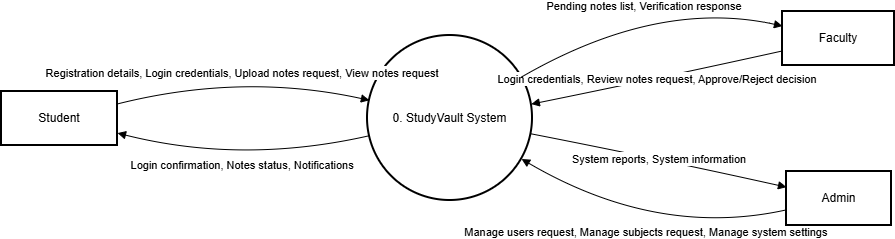
\includegraphics[width=0.8\textwidth]{dfd_level0.png}
\caption{Level 0 Data Flow Diagram (Context Diagram)}
\label{fig:dfd0}
\end{figure}

\section{Level 1 Data Flow Diagram}

The Level~1 DFD decomposes the central StudyVault process into six sub-processes: (1)~User Authentication, (2)~Notes Upload, (3)~AI Safety Analysis, (4)~Faculty Verification, (5)~Notes Management, and (6)~Notification System. Data stores include the Users, Notes, Notifications, and Messages collections in MongoDB.

\begin{figure}[H]
\centering
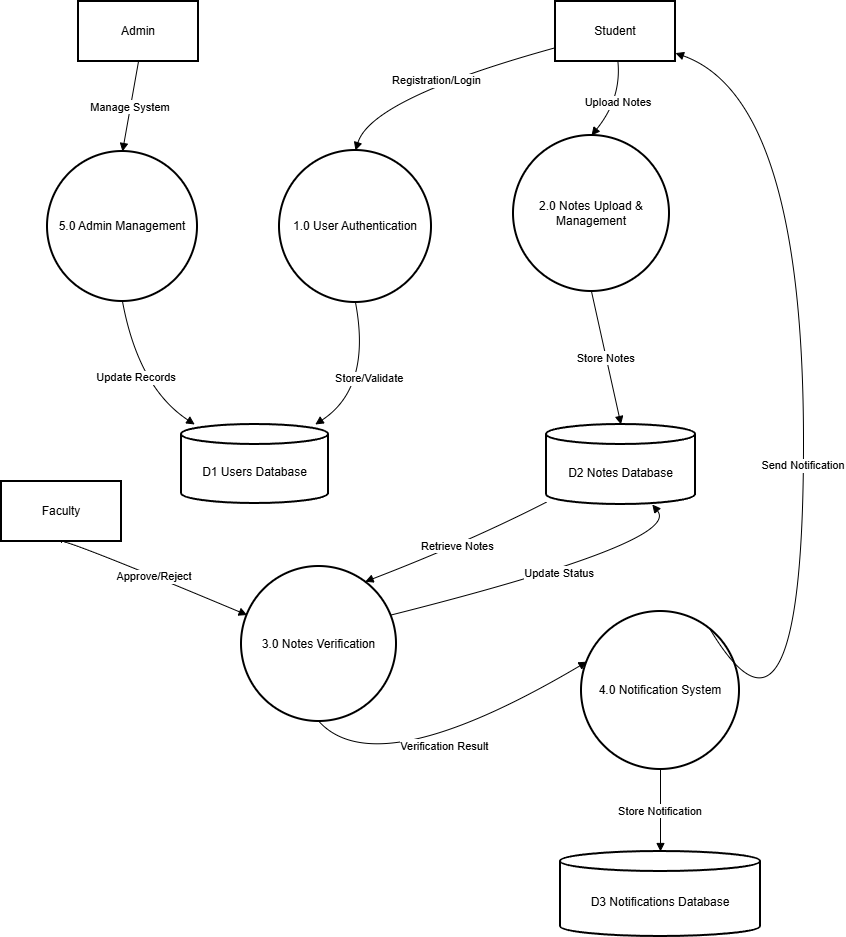
\includegraphics[width=0.8\textwidth]{dfd_level1.png}
\caption{Level 1 Data Flow Diagram}
\label{fig:dfd1}
\end{figure}

\section{Use Case Diagram}

The Use Case Diagram illustrates the interactions of the three system actors---Student, Faculty, and Admin---with the platform's use cases. Students upload notes, browse and download approved content, and use AI tools. Faculty review and approve notes. The Admin manages users, content, and system settings.

\begin{figure}[H]
\centering
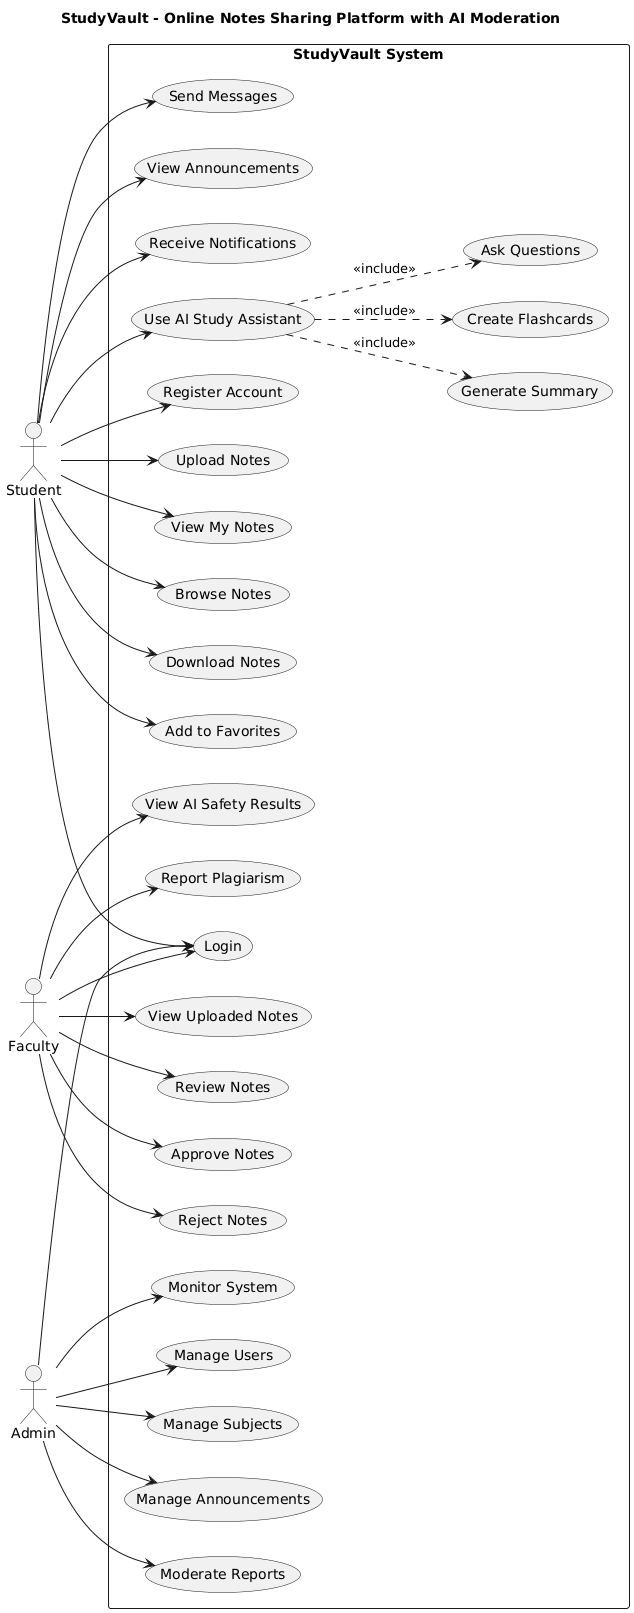
\includegraphics[width=0.8\textwidth]{use_case_diagram.png}
\caption{Use Case Diagram of StudyVault}
\label{fig:usecase}
\end{figure}

\section{Database Schema}

StudyVault uses a MongoDB NoSQL database named \texttt{studyvault}. The schema comprises nine collections: \texttt{users}, \texttt{notes}, \texttt{favorites}, \texttt{notifications}, \texttt{messages}, \texttt{forum\_posts}, \texttt{announcements}, \texttt{reports}, and \texttt{system\_settings}. Each collection stores documents specific to a domain of the application.

\begin{figure}[H]
\centering
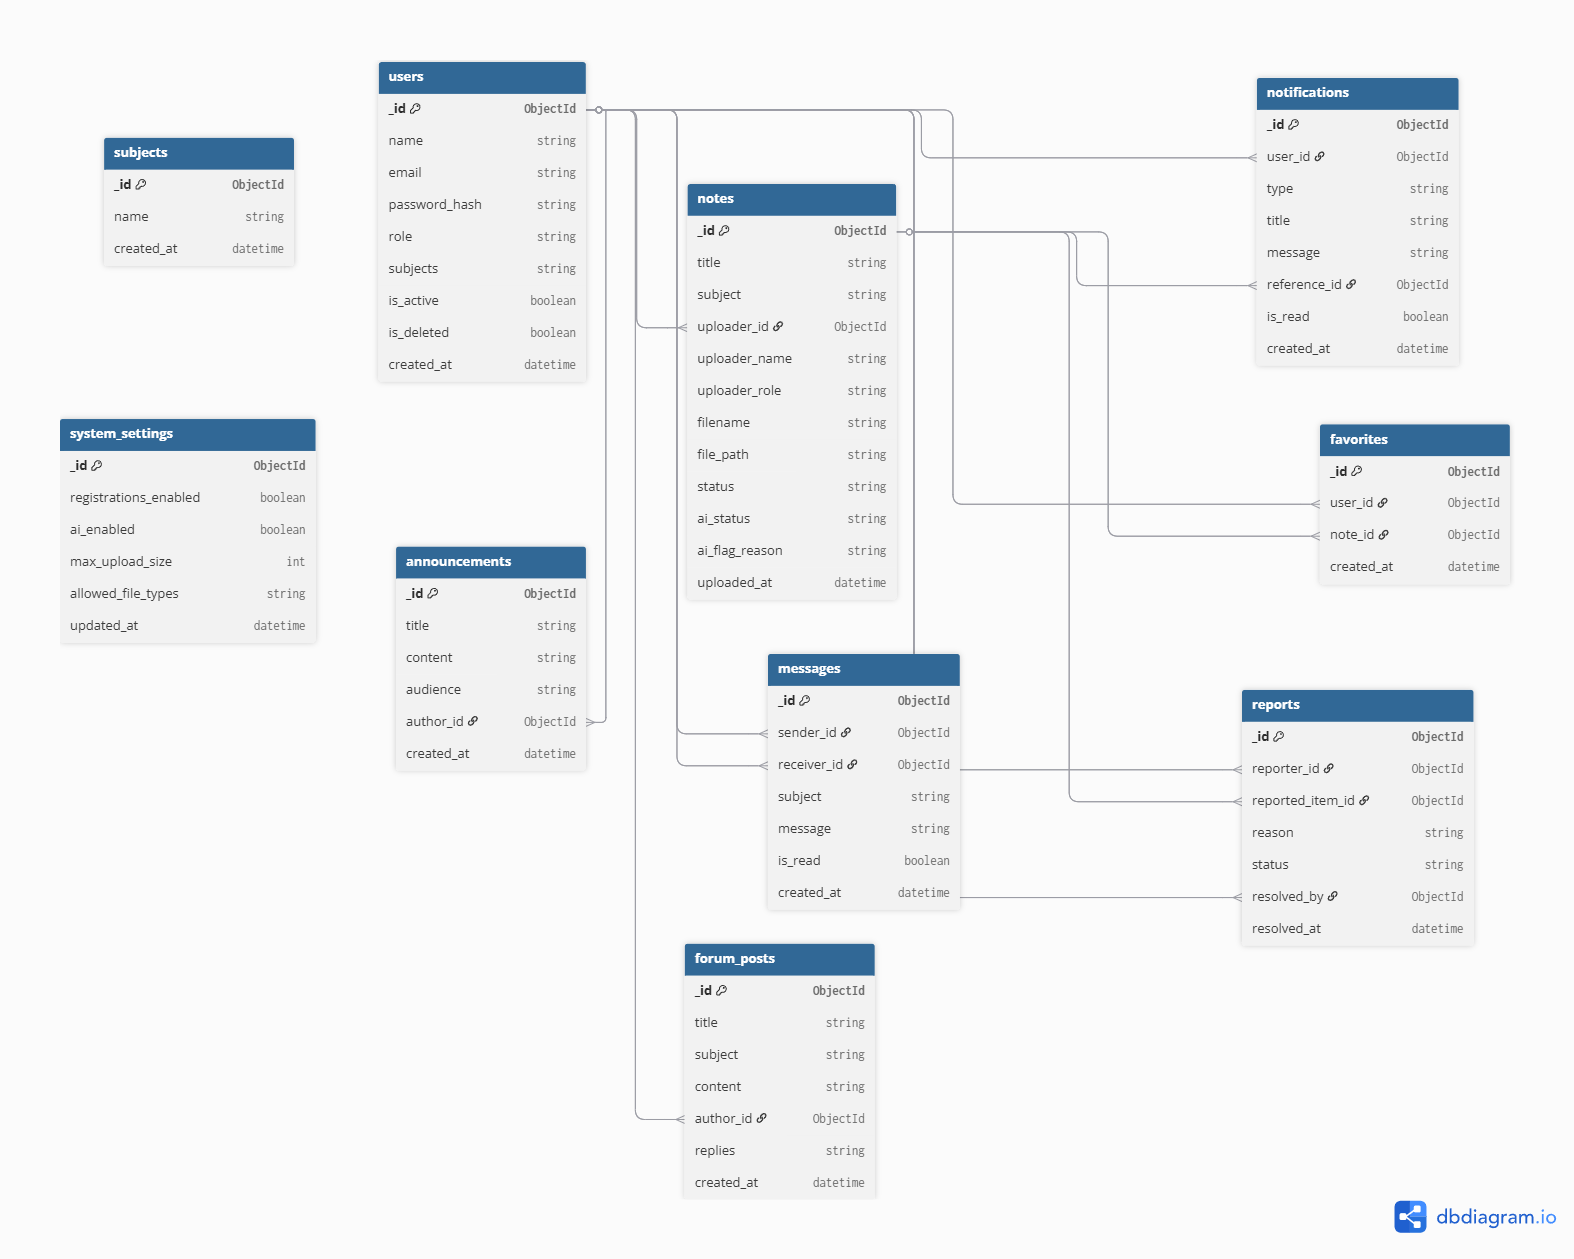
\includegraphics[width=0.8\textwidth]{database_schema.png}
\caption{Database Schema of StudyVault}
\label{fig:schema}
\end{figure}

The \texttt{users} collection stores authentication credentials, role, and profile data. The \texttt{notes} collection stores the full lifecycle of a note---from upload through AI screening, faculty decision, and publication. The \texttt{notifications} collection enables the real-time bell-badge system. The \texttt{system\_settings} collection allows the administrator to configure platform behaviour without any code changes.

\section{Implementation}

\subsection{Backend}

The backend of StudyVault is built using \textbf{FastAPI}, a modern Python ASGI web framework, served by \textbf{Uvicorn}. The application is divided into modular routers, each responsible for a distinct role domain:

\begin{itemize}
    \item \texttt{auth.py} -- Role selection, registration with bcrypt password hashing, session-based login, and logout.
    \item \texttt{student.py} -- Dashboard, multi-file upload, AI safety pipeline trigger, browse, download, favourites, messaging, discussion forum, AI tools, notifications, and announcements.
    \item \texttt{faculty.py} -- Approval queue (tabbed by status), approve/reject/return actions, note preview, faculty uploads, announcements, and messaging.
    \item \texttt{admin.py} -- User management (activate/deactivate/soft-delete), note moderation, report resolution, announcements, messaging, analytics dashboard, and system settings.
    \item \texttt{reports.py} -- Content reporting by any user; triggers a notification to admin and flags content for investigation.
\end{itemize}

\textbf{AI Integration} uses the Groq Python client to call the \texttt{llama-3.1-8b-instant} model. Text is first extracted from uploaded files---PyPDF2 for PDFs, pytesseract for images, python-docx or python-pptx for Office documents---then passed to the Groq API with a structured system prompt that requests a JSON safety report scoring six violation categories each on a scale of 0--10, plus an overall verdict of ``Safe'' or ``Flagged''. All AI calls run inside \texttt{asyncio.to\_thread()} to prevent blocking the ASGI event loop.

\textbf{Database} connectivity uses \textbf{PyMongo}. The \texttt{database.py} module initialises the client, exposes all collection references, creates required indexes (unique email, composite unique favourite), and provides the \texttt{create\_notification()} utility called by every other module.

A custom \textbf{NotificationMiddleware} intercepts every HTTP request and, for logged-in sessions, queries the unread notification count and attaches it to \texttt{request.state.unread\_count}. Jinja2 templates render this value as a badge on the notification bell, updated on every page load without any polling.

\subsection{Frontend}

The frontend is rendered with \textbf{Jinja2} server-side templates. Each role has a dedicated base layout template that supplies the navigation bar, notification bell, and user profile information. Pages extend this base template and override the content block.

The \textbf{Student Dashboard} displays summary statistics (total uploads, approved count, pending count, favourites), the latest faculty announcement as a banner, and a recent activity panel listing the five most recent notifications.

The \textbf{Faculty Dashboard} provides a tabbed approval queue (Pending\,/\,Approved\,/\,Rejected), inline Approve/Reject/Return action buttons powered by AJAX fetch calls, an AI Safety modal showing the detailed six-category scores for any selected note, and a performance panel showing average, fastest, and slowest review times.

The \textbf{Admin Dashboard} shows real-time platform metrics---total users, note counts by status, a 7-day upload activity chart, and a faculty analytics table with per-faculty review counts and queue sizes.

JavaScript is used selectively for AJAX interactions (approval actions, AI tool requests), theme toggling, and dynamic rendering of AI tool responses. No JavaScript framework is used; all logic is plain ES6.

% ============================================================
%  CHAPTER 4 – TESTING
% ============================================================
\chapter{TESTING}

\section{Testing Approach}

Testing was performed manually in three phases. First, individual routes and functions were tested independently using direct browser access and Postman for POST endpoints. Second, each feature was tested end-to-end through the browser interface with all three user roles. Third, input forms were tested with missing, invalid, and boundary-case values. Error responses and edge cases were validated by checking browser output, server console logs, and MongoDB collection states.

Types of testing performed include: Functional Testing, Validation Testing, Security Testing (cross-role login, timing attack resistance), Module Testing, and Boundary Testing (file type enforcement, empty submissions, very large AI inputs).

\section{Black Box Test Cases}

\begin{table}[H]
\centering
\small
\begin{tabular}{|p{1.5cm}|p{3cm}|p{2.5cm}|p{3cm}|p{2.5cm}|p{1.2cm}|}
\hline
TC ID & Description & Input & Expected Output & Result & Status \\
\hline
TC01 & Student registration & Valid name, email, password & Redirect to login & Success & Pass \\
\hline
TC02 & Login wrong password & Valid email, wrong password & Error message & Error shown & Pass \\
\hline
TC03 & Cross-role login & Student login in faculty portal & Access denied & Denied & Pass \\
\hline
TC04 & Duplicate email & Existing email & Registration blocked & Error shown & Pass \\
\hline
TC05 & Deactivated account login & Inactive account & Access denied & Login failed & Pass \\
\hline
TC06 & Upload valid PDF & PDF upload & Note created & Stored in DB & Pass \\
\hline
TC07 & Upload invalid file & .exe file & File rejected & Skipped & Pass \\
\hline
TC08 & Upload without login & POST request & Redirect to login & Redirected & Pass \\
\hline
TC09 & Upload multiple files & 3 files & 3 records created & Stored & Pass \\
\hline
TC10 & Approve note & Faculty approve & Status approved & Updated & Pass \\
\hline
TC11 & Reject note & Faculty reject & Status rejected & Stored & Pass \\
\hline
TC12 & Download note & Download click & File served & Success & Pass \\
\hline
TC13 & Toggle favourite & Heart icon click & Note saved & Success & Pass \\
\hline
TC14 & Create announcement & Valid markdown input & Announcement posted & Success & Pass \\
\hline
TC15 & Deactivate user & Admin clicks toggle & Account locked out & Success & Pass \\
\hline
\end{tabular}
\caption{Black Box Test Cases for StudyVault}
\end{table}

\section{Error Handling and Validation}

\textbf{Form Validation:} FastAPI uses Pydantic to validate all form data types. Missing required fields return HTTP~422 with detailed error descriptions.

\textbf{Session Checks:} Every route begins with a role-check helper---\texttt{get\_current\_student()}, \texttt{get\_current\_faculty()}, or \texttt{get\_current\_admin()}. If the check fails, the user is immediately redirected to \texttt{/login}.

\textbf{Database Safety:} A \texttt{safe\_id()} helper wraps all ObjectId conversions in try-except blocks to prevent crashes from malformed ID strings in URL parameters.

\textbf{AI Failures:} All Groq API calls are wrapped in try-except. On any exception, a safe fallback dictionary is returned so the upload is not blocked by an AI service failure.

% ============================================================
%  CHAPTER 5 – RESULTS
% ============================================================
\chapter{RESULTS}

\section{Role Selection Page}

Users are presented with a role selection screen on first visiting the platform. Selecting a role redirects to the corresponding login form. Cross-role logins are blocked at the server and a generic error is returned.

\begin{figure}[H]
\centering

\includegraphics[width=0.85\textwidth]{role_selection.png}
\caption{Role Selection Page}
\label{fig:roleselection}
\end{figure}

\section{Login Page}

The login page is specific to the selected role. Session is maintained server-side using the Starlette SessionMiddleware. Constant-time password verification prevents timing-based email enumeration.

\begin{figure}[H]
\centering
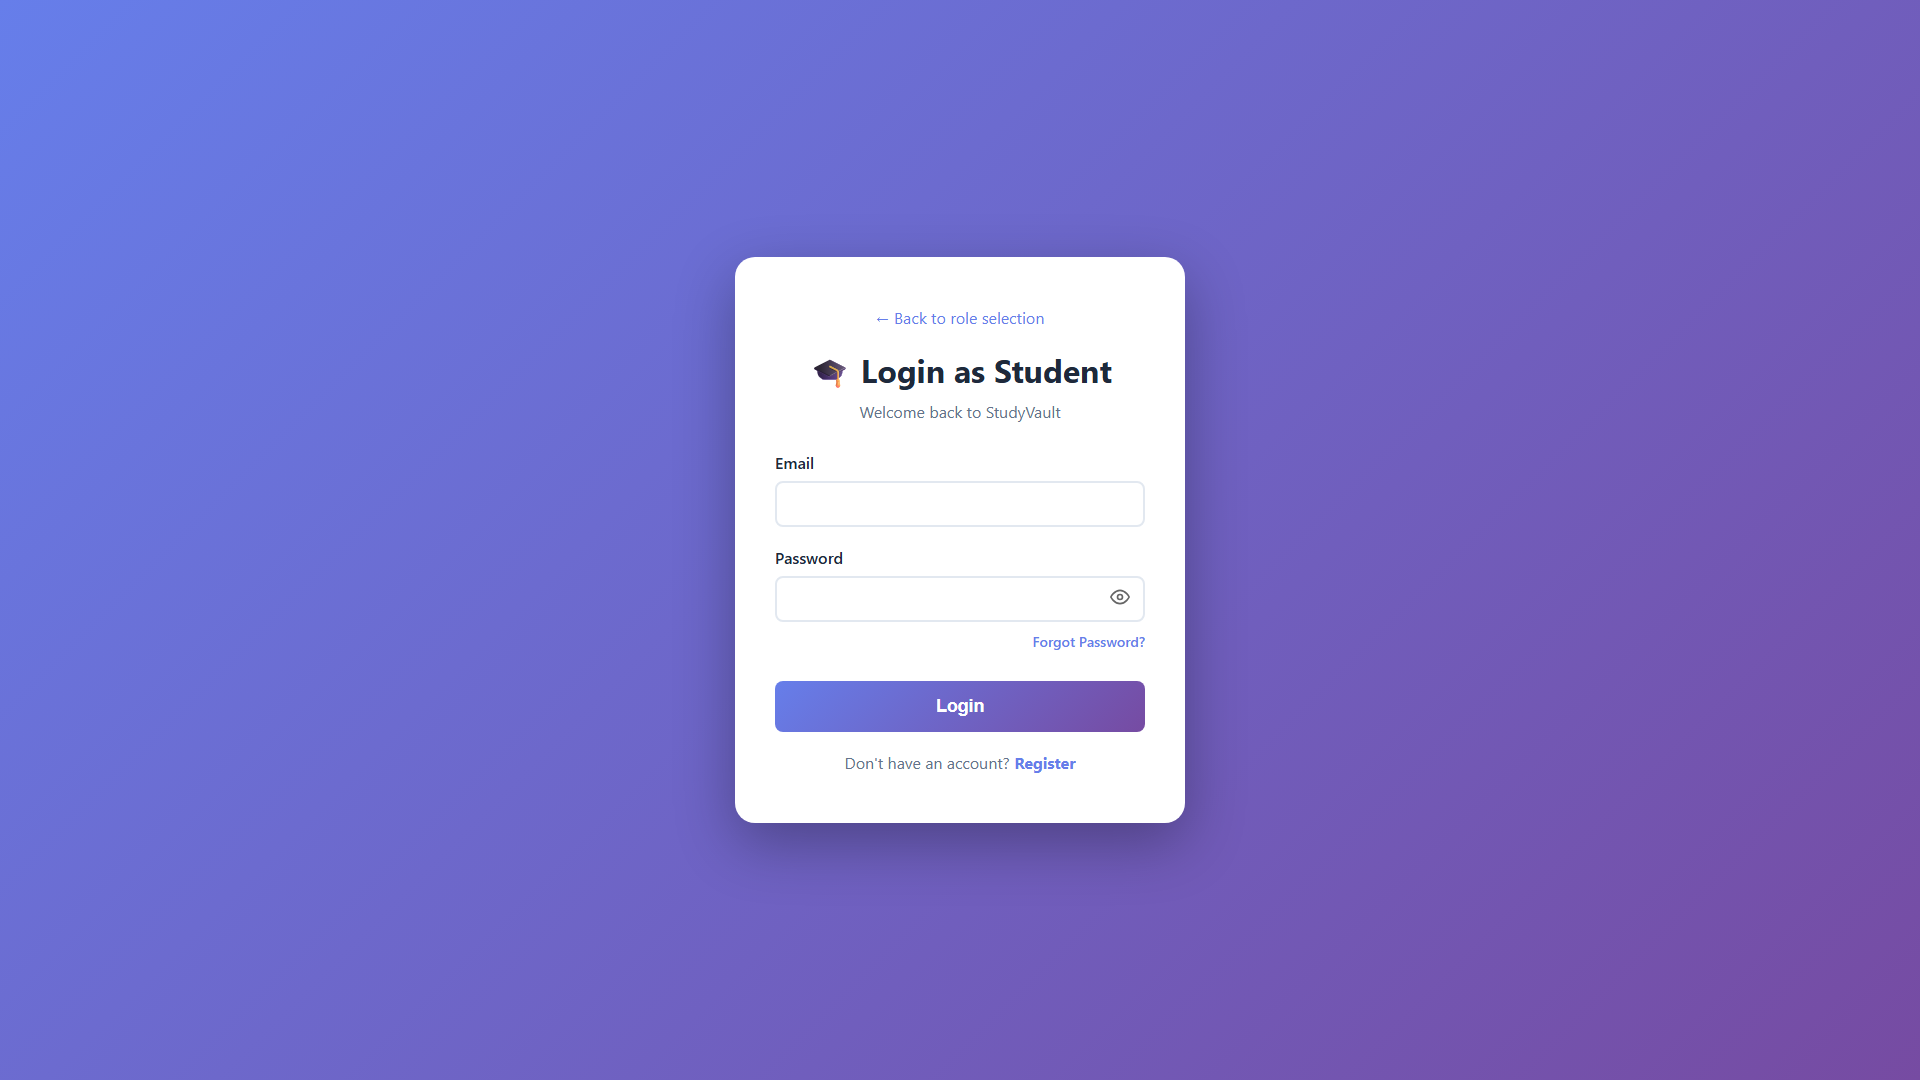
\includegraphics[width=0.85\textwidth]{login_page.png}
\caption{Login Page}
\label{fig:login}
\end{figure}

\section{Student Dashboard}

The student dashboard displays real-time statistics: total uploads, approved note counts, pending notes, and saved favourites. The latest faculty announcement is shown as a banner and recent activity is listed in a notification panel.

\begin{figure}[H]
\centering
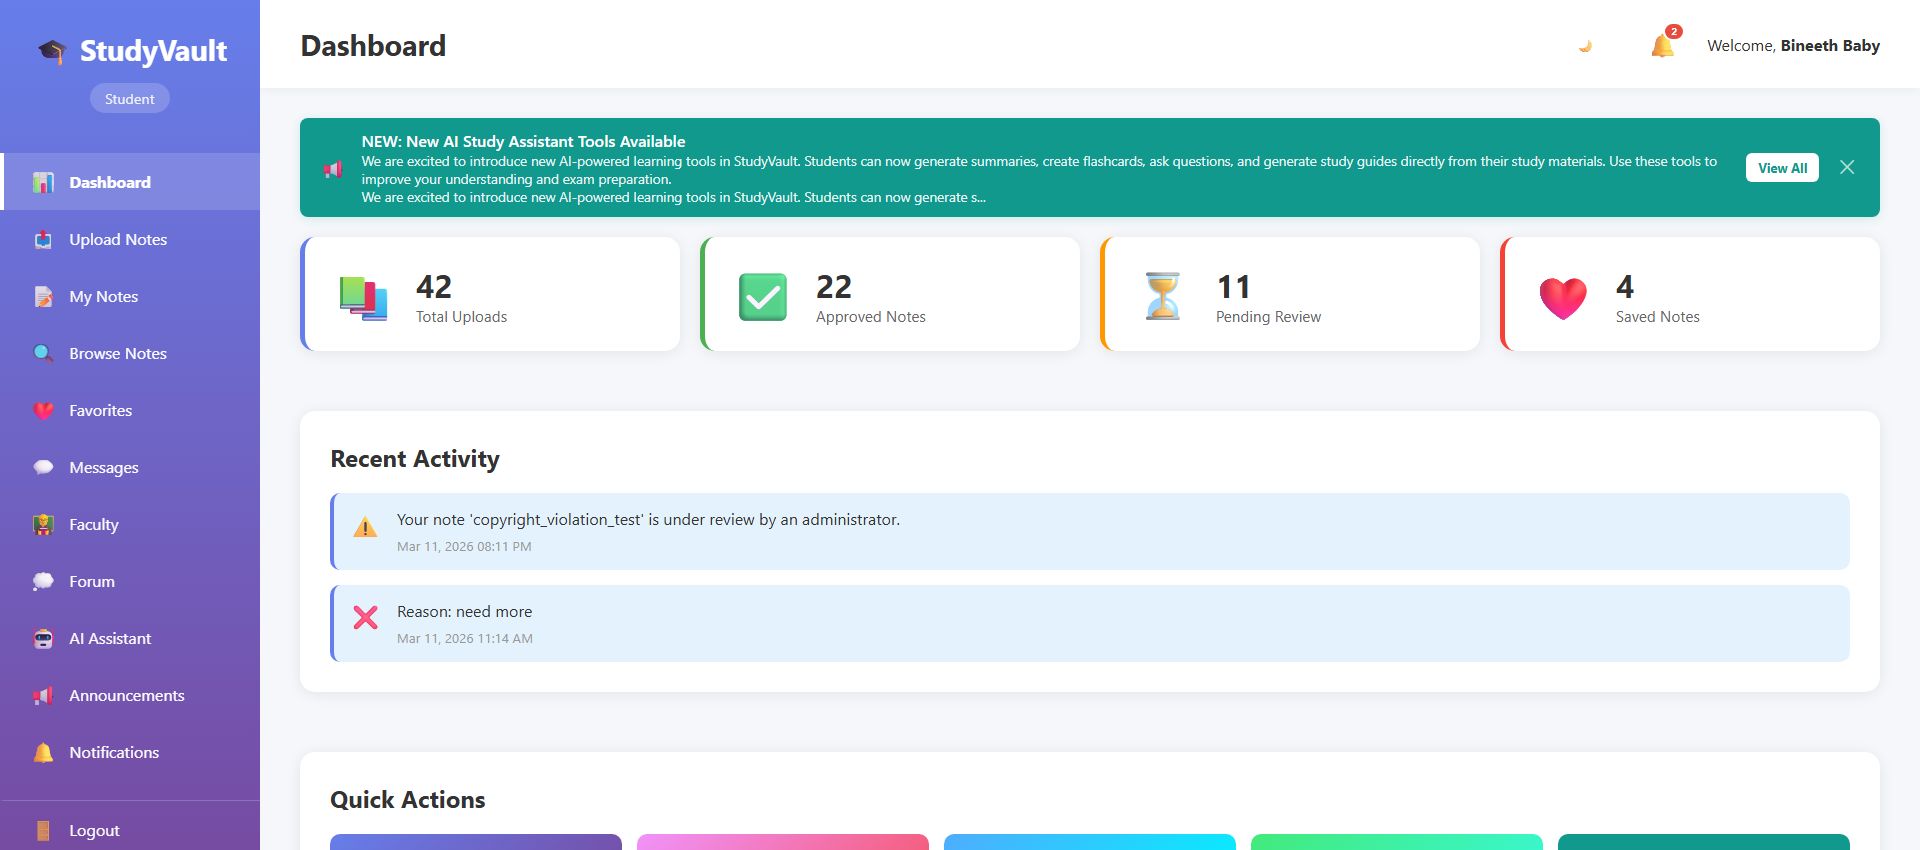
\includegraphics[width=0.85\textwidth]{student_dashboard.png}
\caption{Student Dashboard}
\label{fig:studentdash}
\end{figure}

\section{Faculty Dashboard}

The faculty dashboard provides a tabbed view of Pending, Approved, and Rejected notes scoped to the faculty member's assigned subjects. Inline Approve\,/\,Reject\,/\,Return actions are AJAX-powered. A performance statistics panel shows average review time.

\begin{figure}[H]
\centering
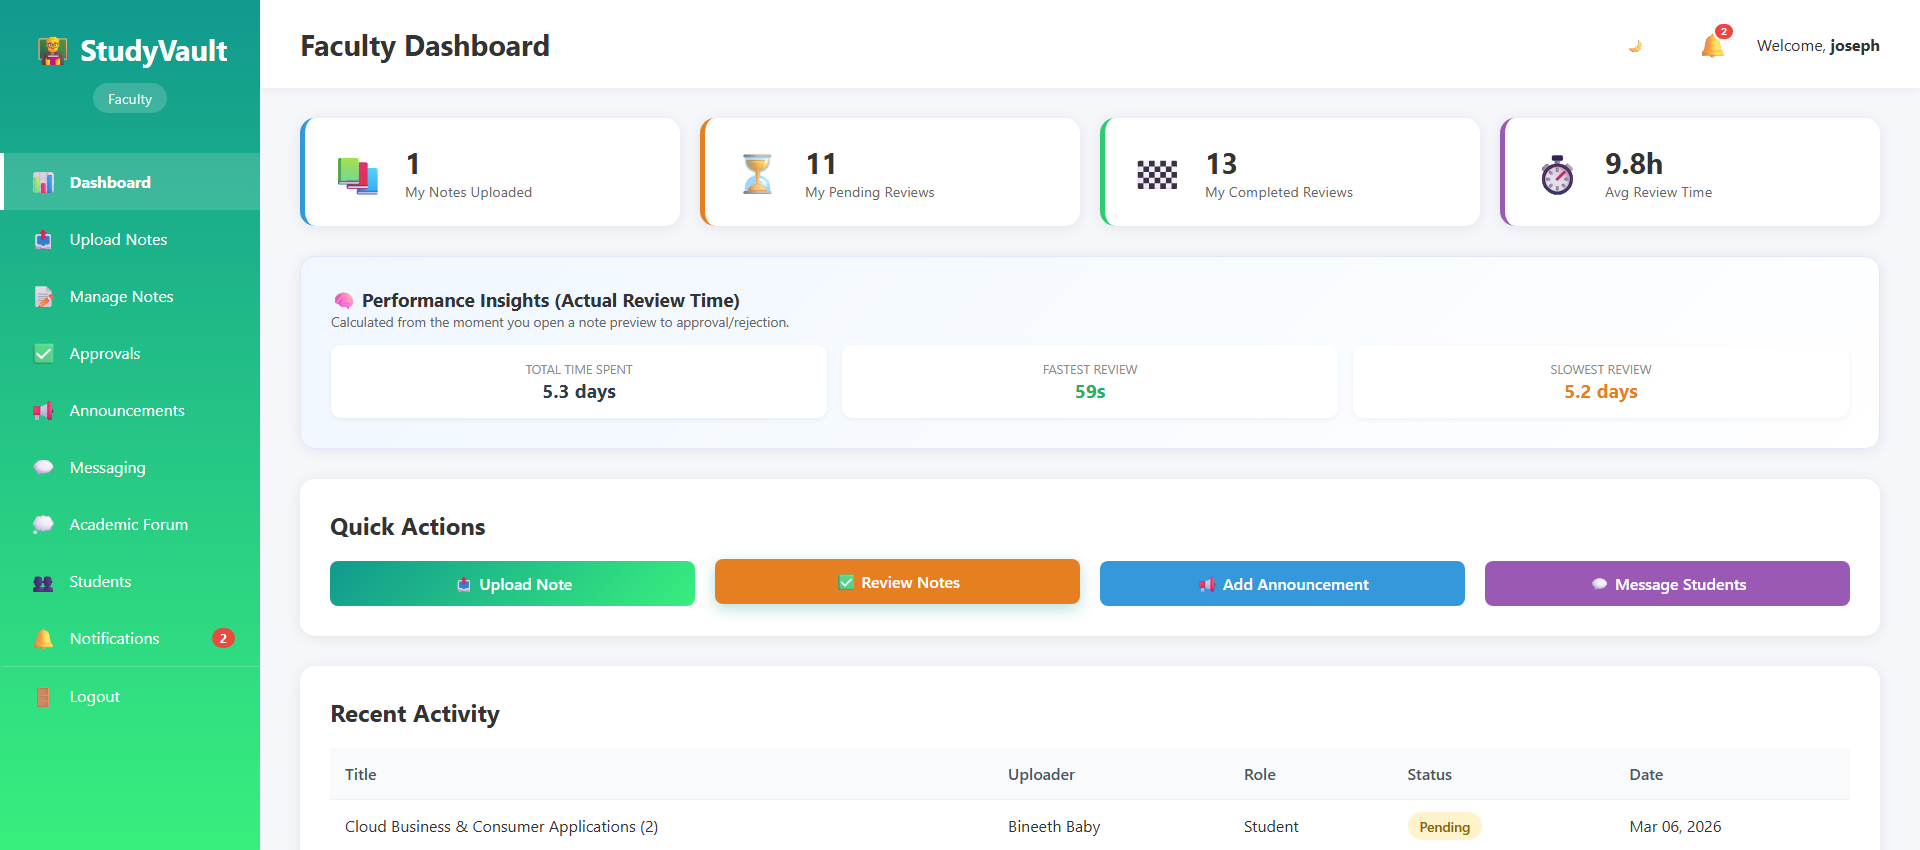
\includegraphics[width=0.85\textwidth]{faculty_dashboard.png}
\caption{Faculty Dashboard}
\label{fig:facultydash}
\end{figure}

\section{Admin Dashboard}

The admin dashboard shows total users, notes by status, a 7-day upload activity chart, a 7-day reports chart, and a faculty analytics table with per-faculty review counts, average review times, and current active status.

\begin{figure}[H]
\centering
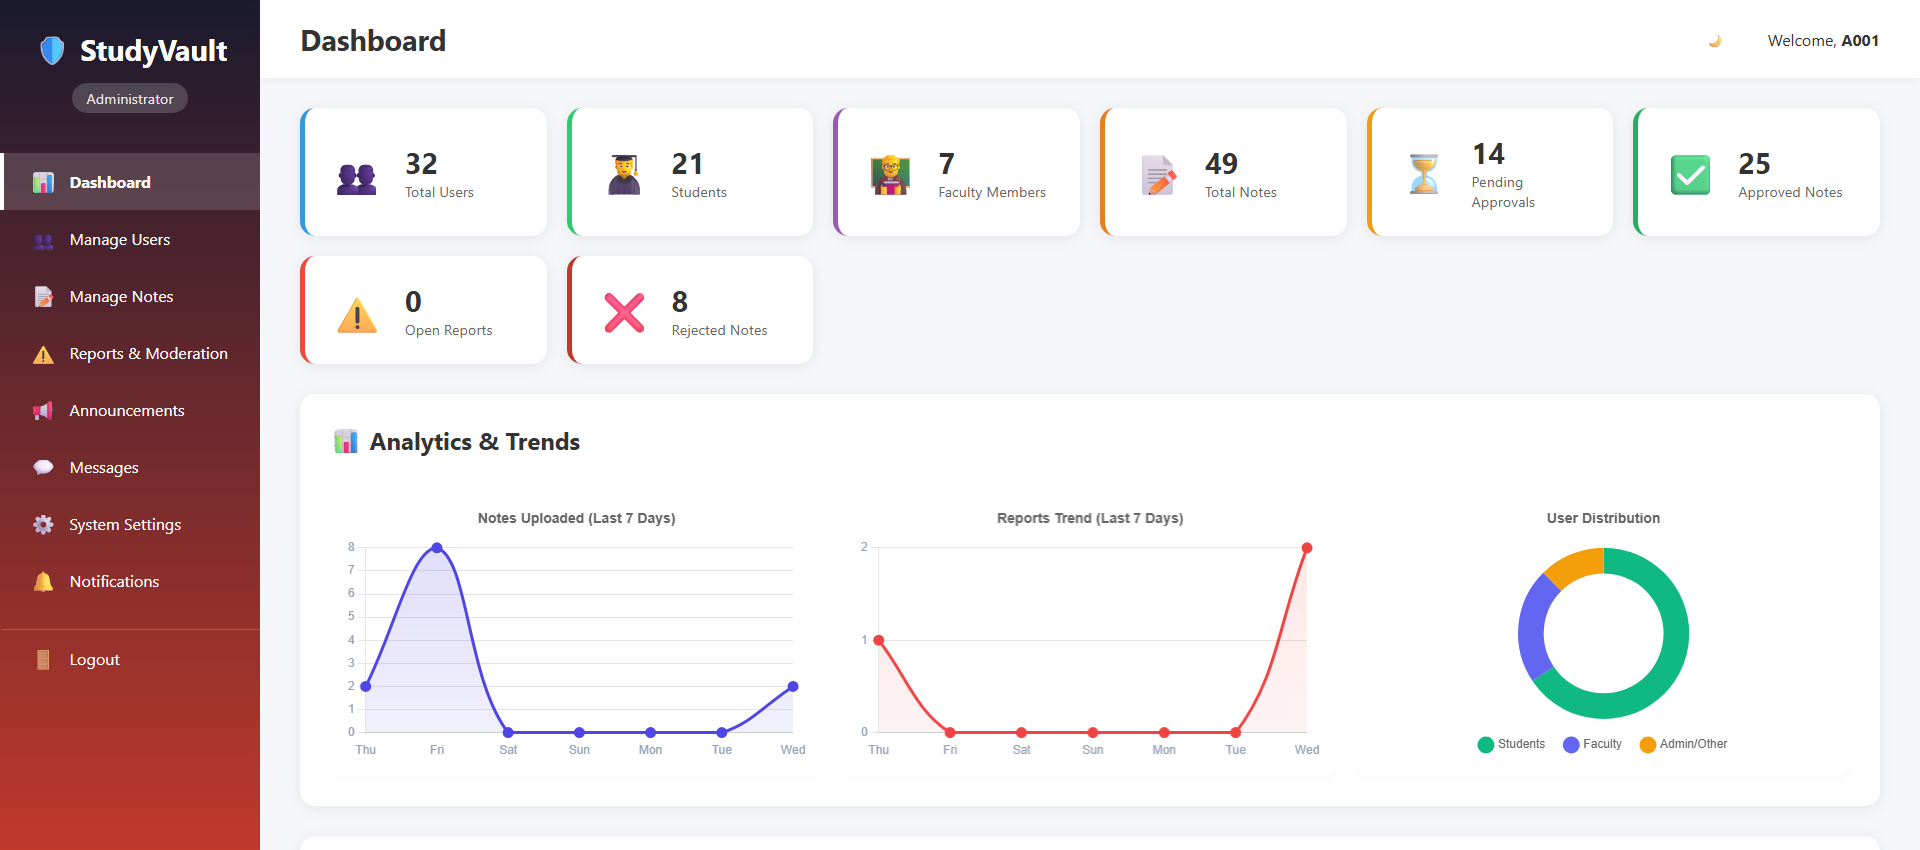
\includegraphics[width=0.85\textwidth]{admin_dashboard.png}
\caption{Admin Dashboard}
\label{fig:admindash}
\end{figure}

\section{Upload Notes Page}

Students upload files using a drag-and-drop interface. Each uploaded file triggers the AI safety pipeline before the note record is created in the database. The AI result is stored alongside the note and is visible to faculty reviewers.

\begin{figure}[H]
\centering
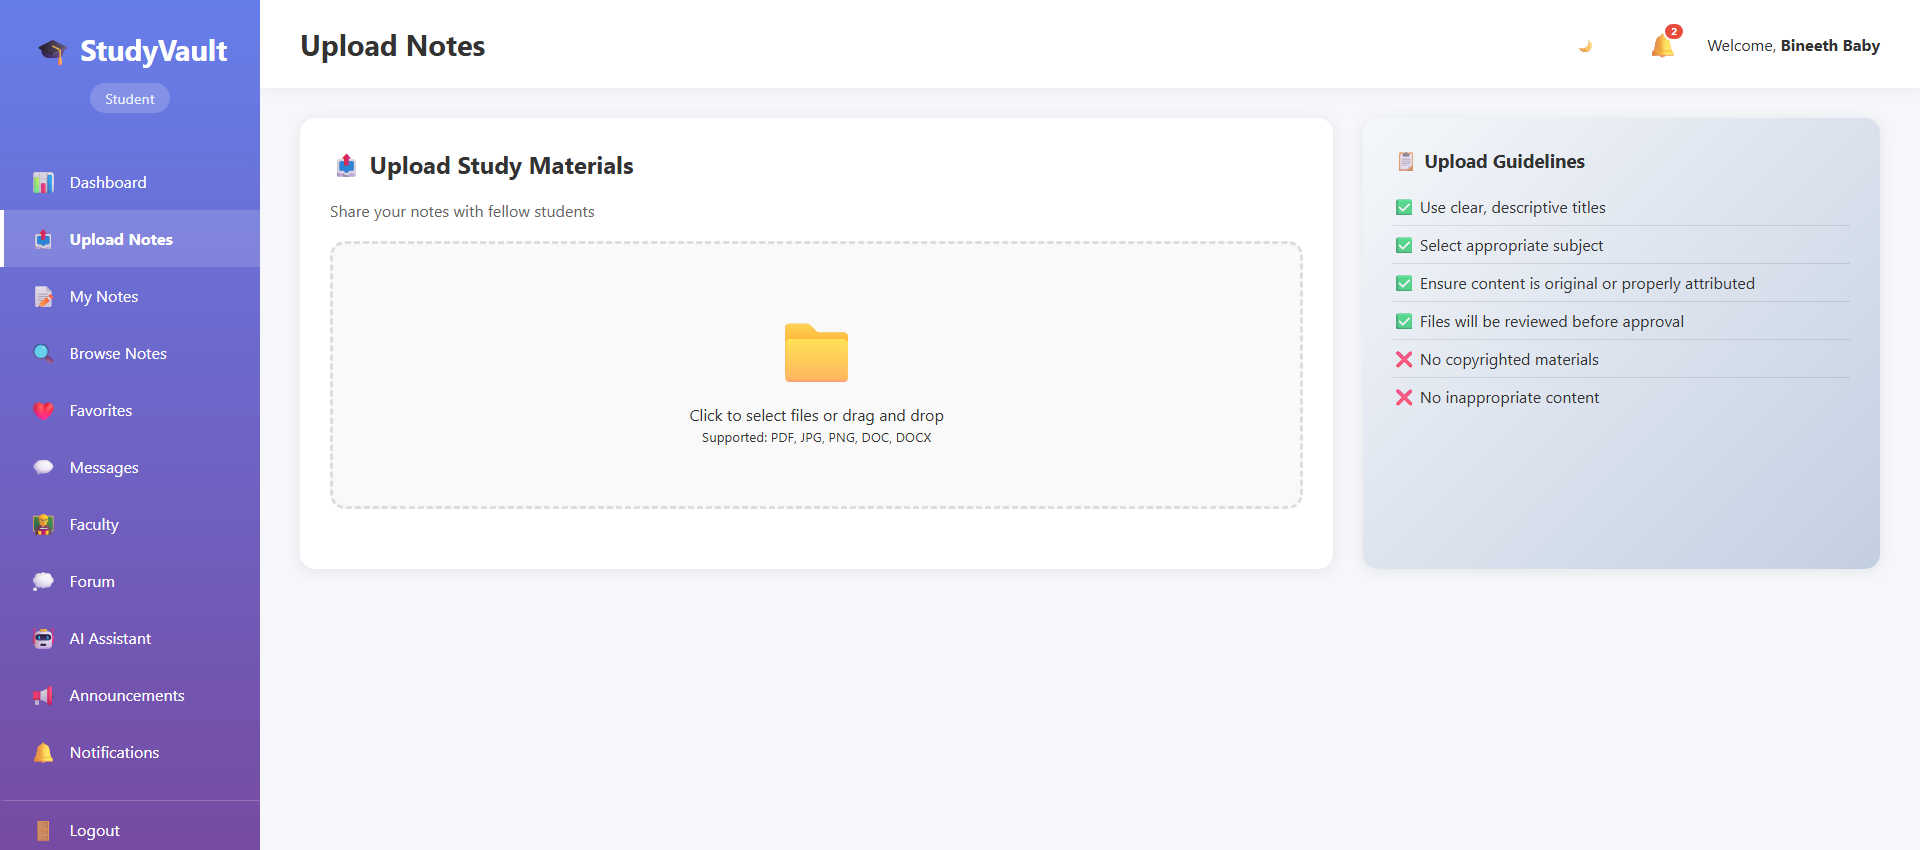
\includegraphics[width=0.85\textwidth]{upload_notes.png}
\caption{Upload Notes Page}
\label{fig:upload}
\end{figure}

\section{Browse Notes Page}

All approved notes appear in the Browse Notes page. Students can filter by subject and search by title. Each note card shows the uploader's name and a heart icon for saving to favourites. A Download button streams the original file.

\begin{figure}[H]
\centering
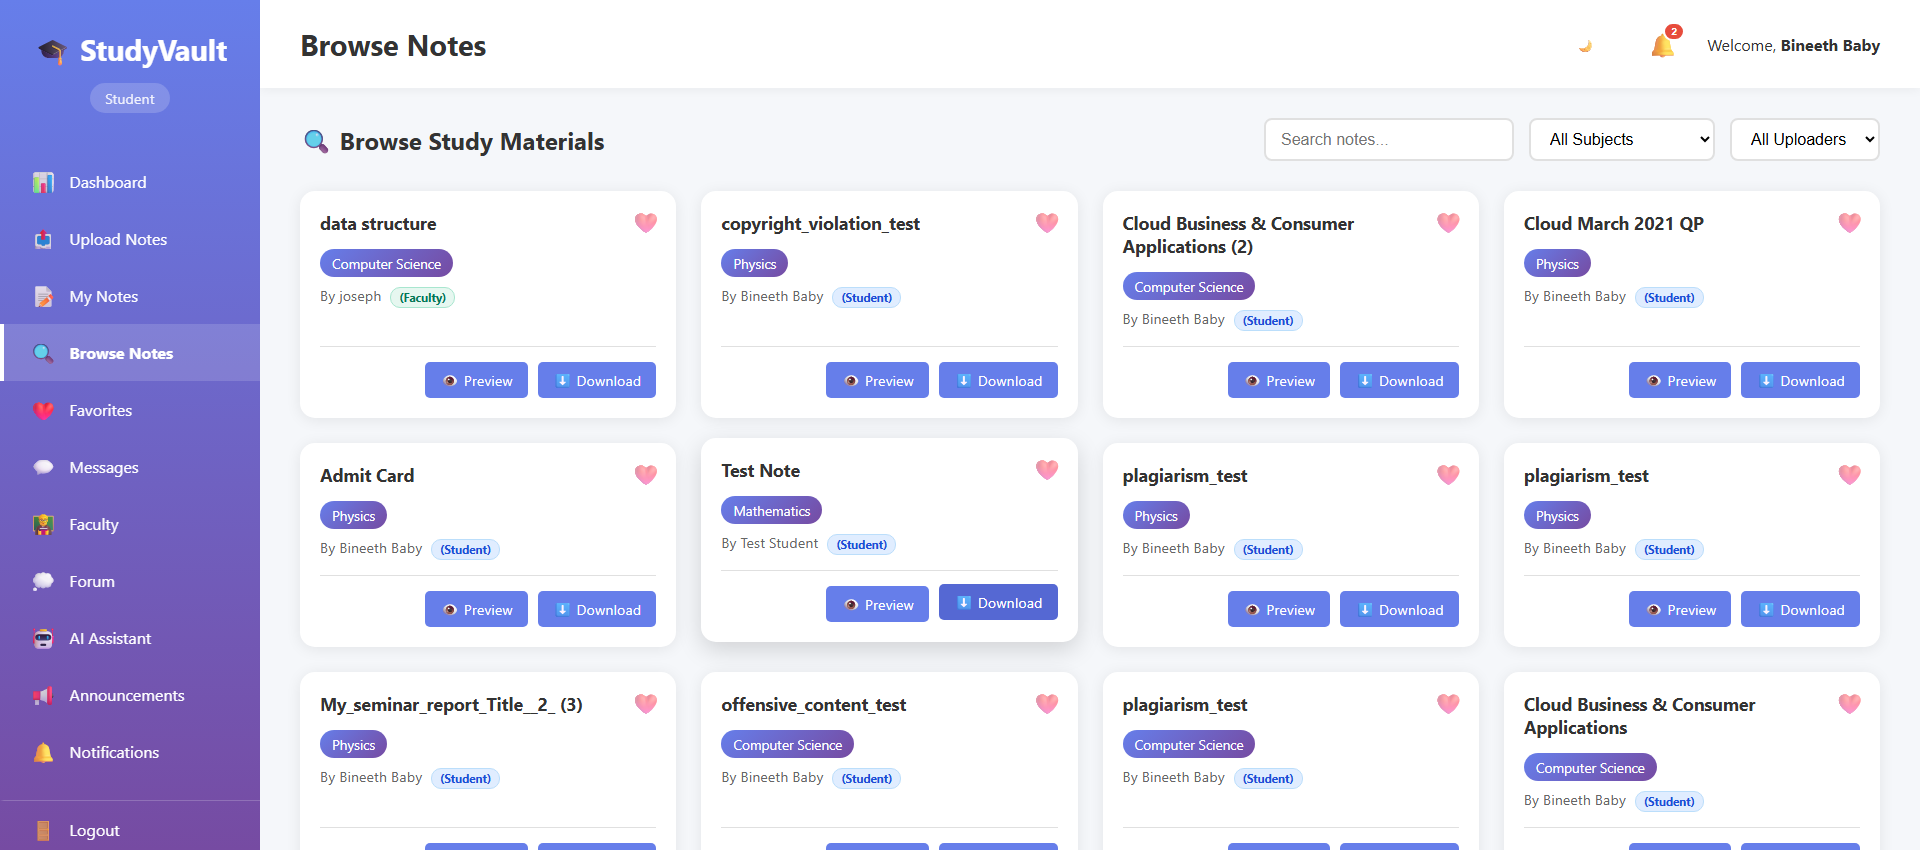
\includegraphics[width=0.85\textwidth]{browse_notes.png}
\caption{Browse Notes Page}
\label{fig:browse}
\end{figure}

\section{Faculty Review Notes Page}

The Faculty Review Notes page shows each note pending review with the AI safety report accessible via a modal. Faculty can Approve, Reject (with a mandatory reason), or Return the note for correction directly from this page.

\begin{figure}[H]
\centering
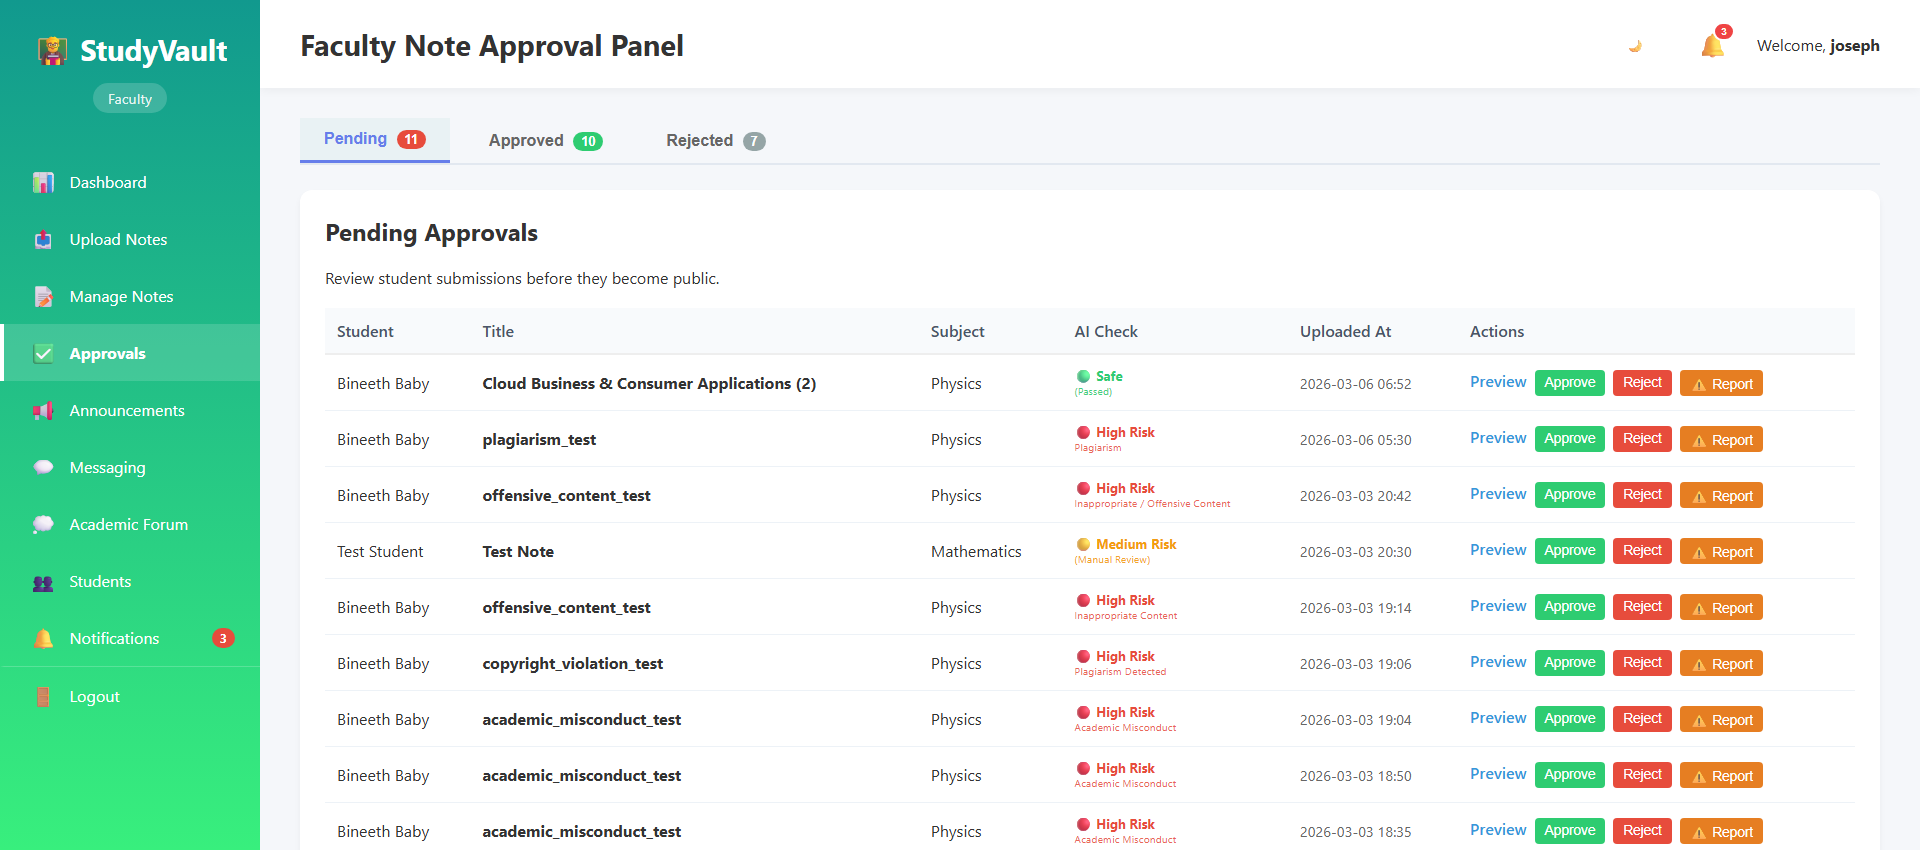
\includegraphics[width=0.85\textwidth]{faculty_review_notes.png}
\caption{Faculty Review Notes Page}
\label{fig:facultyreview}
\end{figure}

\section{Manage Users Page}

The administrator can view all platform users, their roles, join dates, and current status. Users can be activated, deactivated, or soft-deleted. Admin accounts are protected from deletion and are labelled ``Protected''.

\begin{figure}[H]
\centering
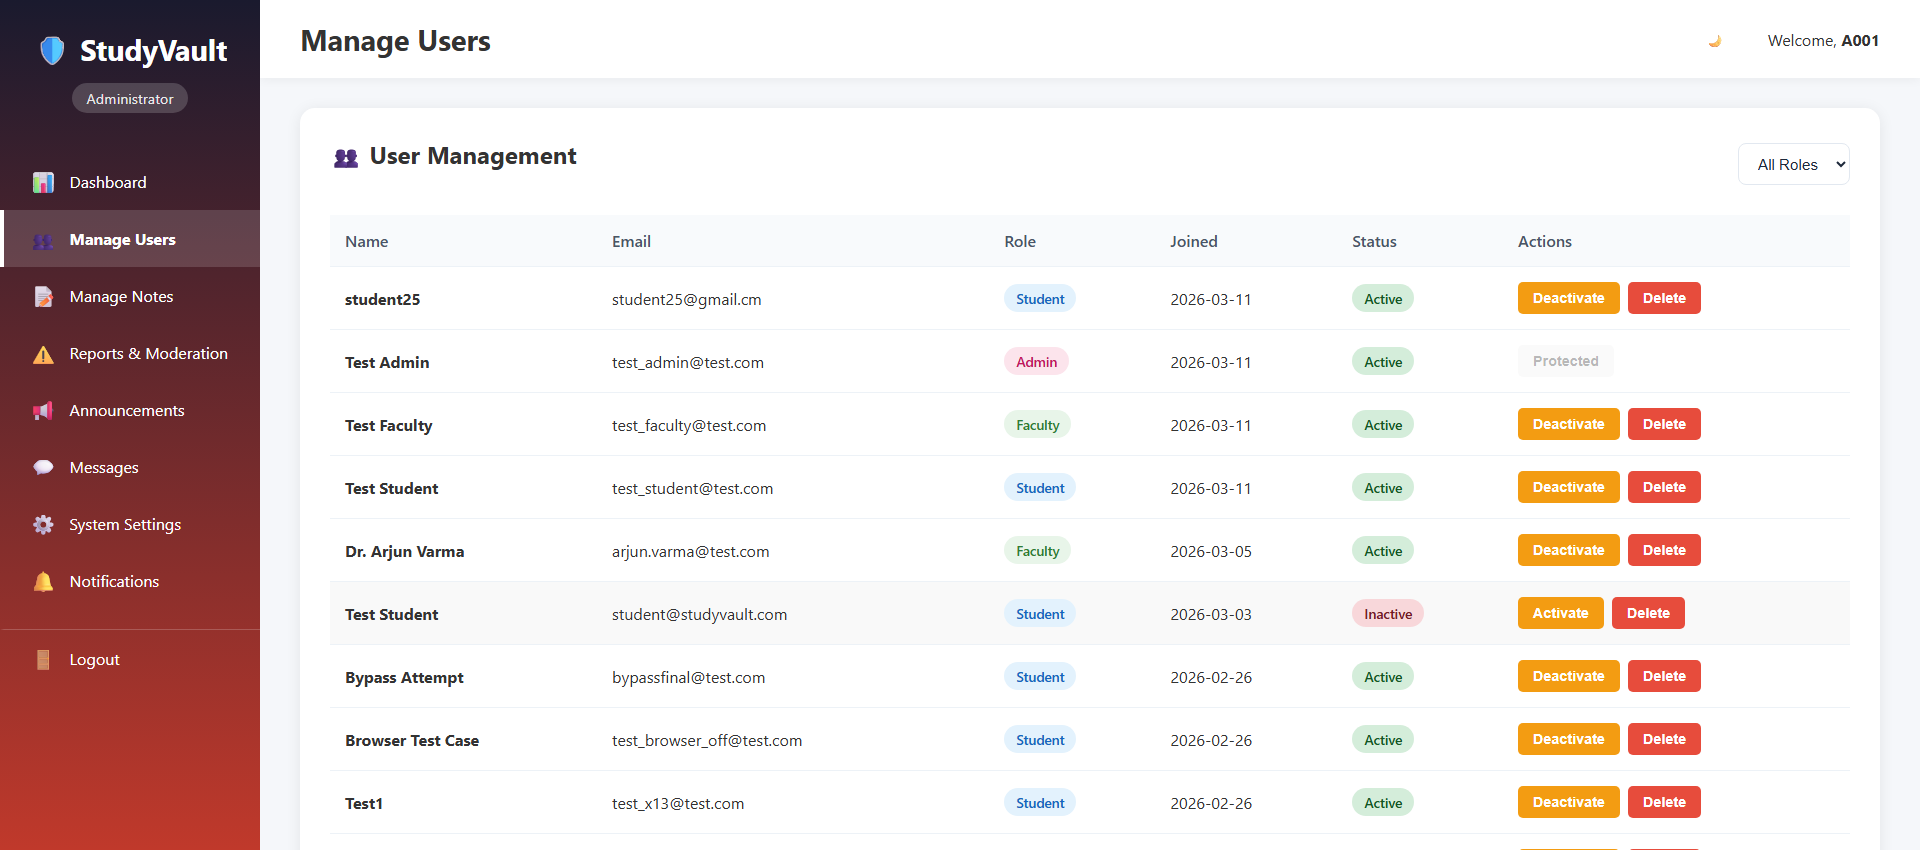
\includegraphics[width=0.85\textwidth]{manage_users.png}
\caption{Manage Users Page}
\label{fig:manageusers}
\end{figure}

\section{Reports and Moderation Page}

The Reports and Moderation page lists all content reports filed by students or faculty. Each report shows the reporter, the reported note, the reason, and the current resolution status. Admins can update status and add a resolution note.

\begin{figure}[H]
\centering
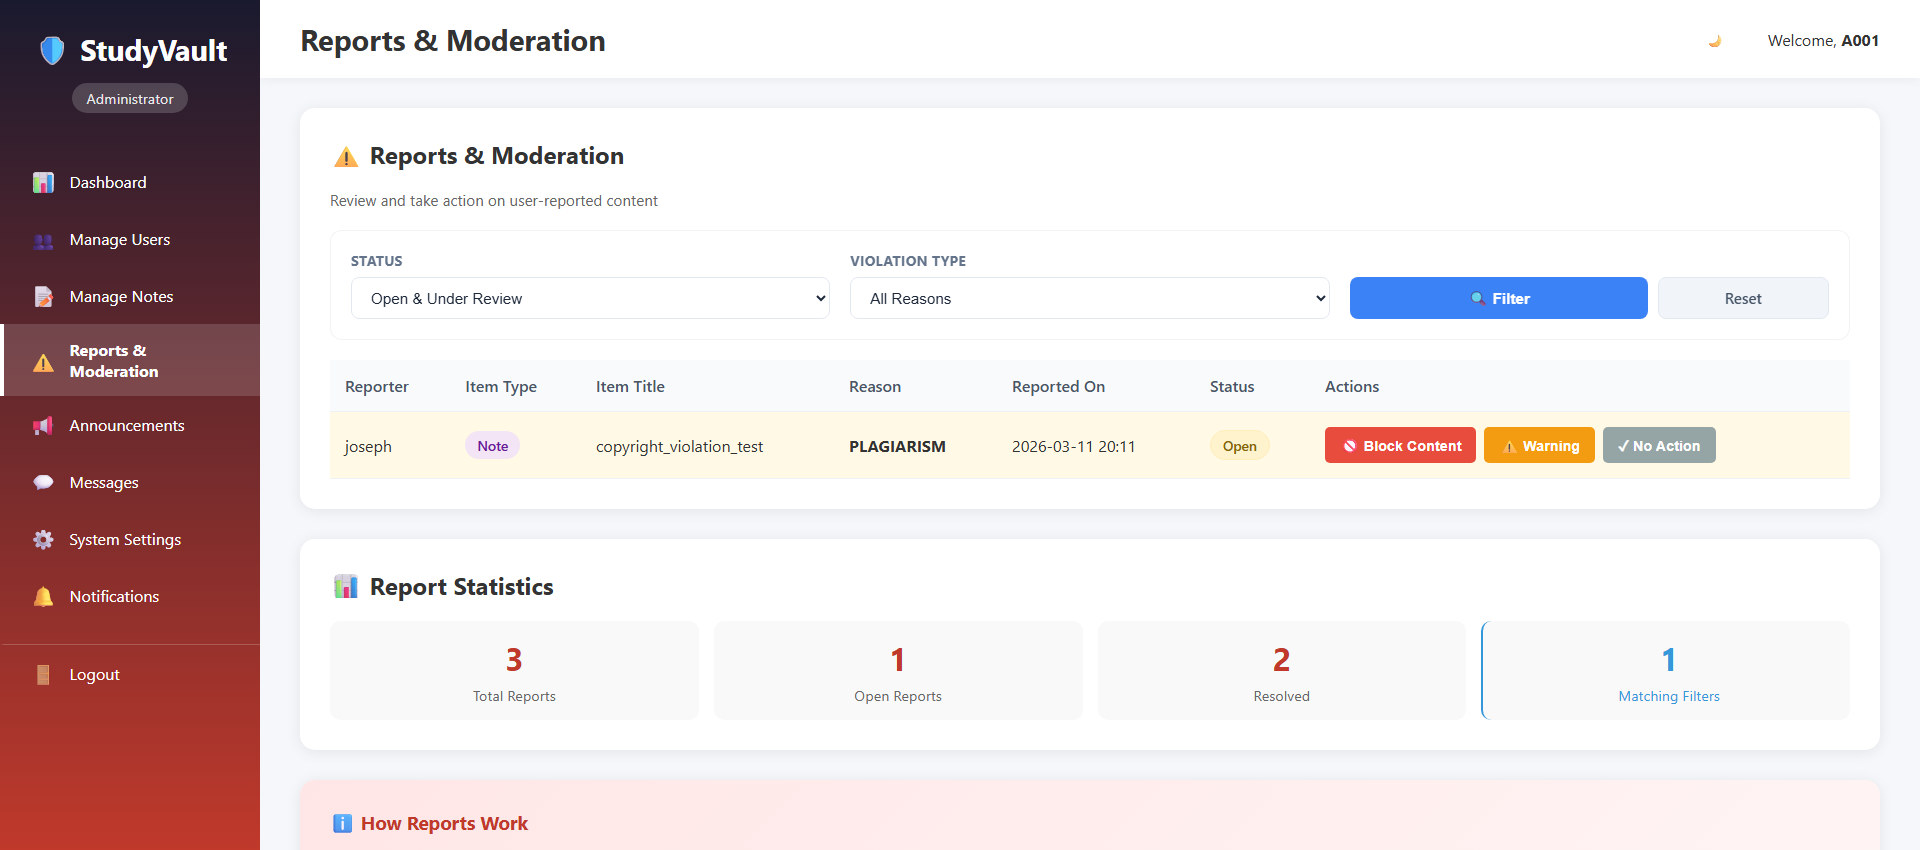
\includegraphics[width=0.85\textwidth]{reports_moderation.png}
\caption{Reports and Moderation Page}
\label{fig:reports}
\end{figure}

\section{AI Assistant Page}

Students paste study text and select a tool---Summary, Flashcards, Q\&A, or Study Guide. Responses are rendered dynamically on the page. Flashcards are displayed as interactive cards. If the API key is unavailable, a demo-mode response is provided gracefully.

\begin{figure}[H]
\centering
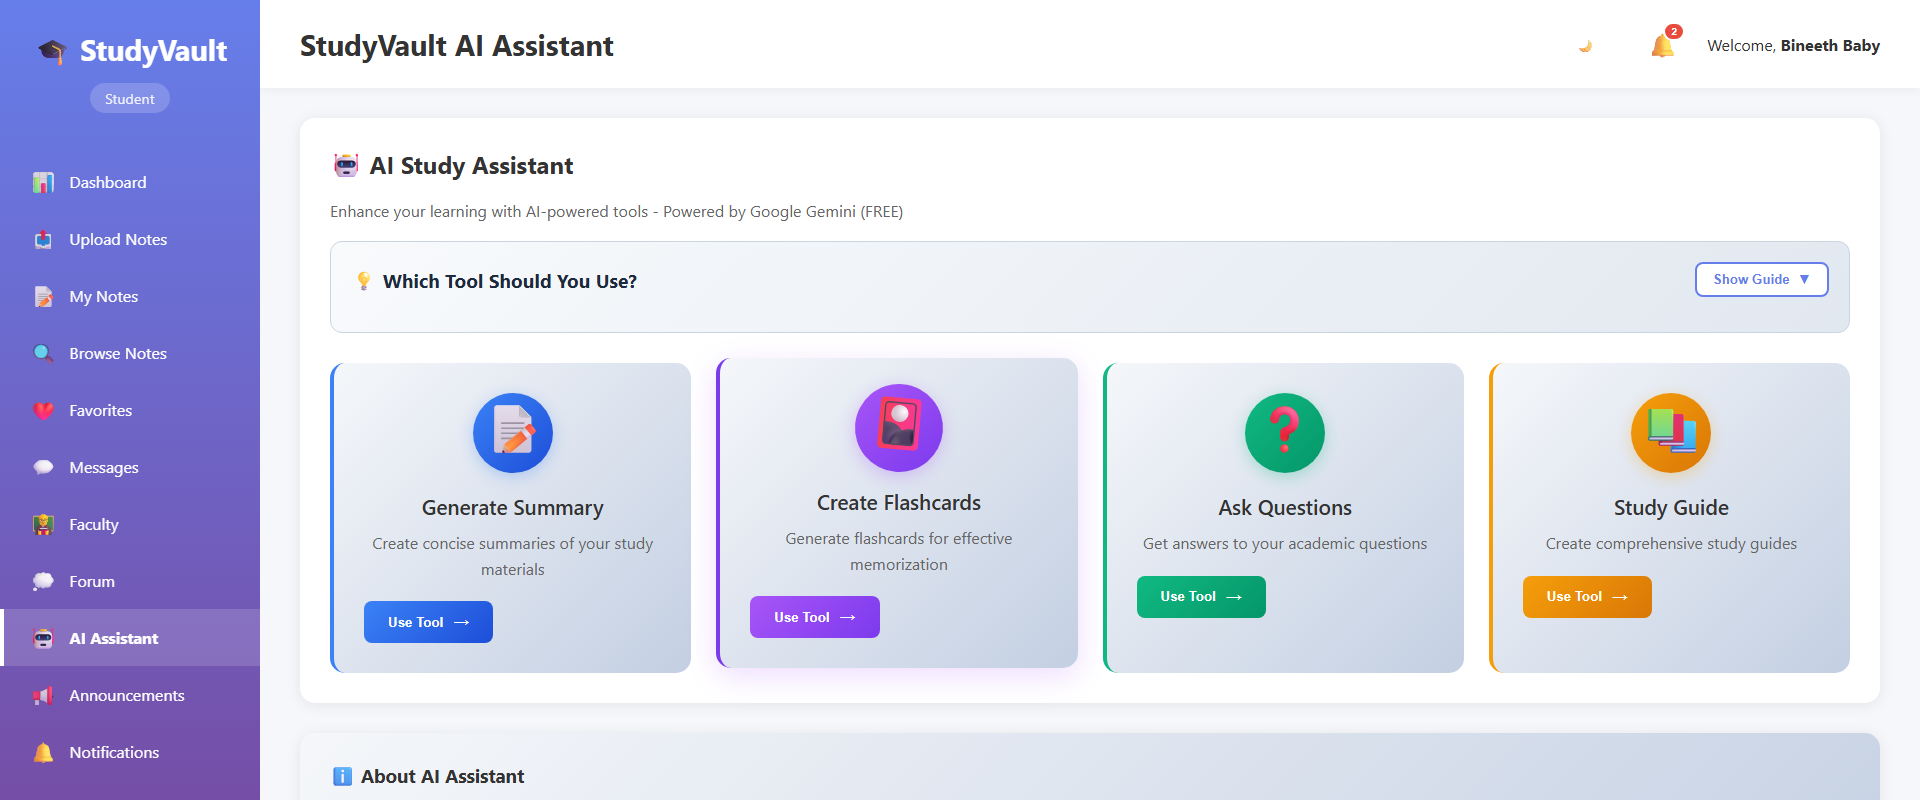
\includegraphics[width=0.85\textwidth]{ai_assistant.png}
\caption{AI Assistant Page}
\label{fig:aiassistant}
\end{figure}

\section{Objectives Achievement Summary}

\begin{table}[H]
\centering
\begin{tabular}{|p{10cm}|p{3cm}|}
\hline
\textbf{Objective} & \textbf{Status} \\
\hline
Secure role-based authentication with bcrypt & Achieved \\
\hline
AI safety analysis on upload via Groq API & Achieved \\
\hline
Faculty review workflow (Approve\,/\,Reject\,/\,Return) & Achieved \\
\hline
Real-time notification system & Achieved \\
\hline
Discussion forum and private messaging & Achieved \\
\hline
Admin user and content management & Achieved \\
\hline
System settings configurable without code changes & Achieved \\
\hline
AI study tools for students & Achieved \\
\hline
\end{tabular}
\caption{Project Objectives Achievement Summary}
\end{table}

All eight primary objectives defined in Chapter~1 were achieved in the final implementation.

% ============================================================
%  CHAPTER 6 – CONCLUSION
% ============================================================
\chapter{CONCLUSION}

\section{Conclusion}

StudyVault successfully demonstrates that it is possible to build a purpose-built, AI-assisted academic notes sharing platform using lightweight modern technologies (FastAPI, MongoDB, Groq API) that is easy to deploy and maintain within an educational institution.

The platform addresses all identified problems of informal, uncontrolled notes sharing by introducing a structured three-tier workflow: student upload, AI pre-screening, and faculty review. The result is a verifiable, high-quality pool of study resources that students and faculty can trust.

The integration of the Groq Llama~3.1 model provides two layers of value: safety (pre-screening uploaded content for six categories of violation) and learning (generating summaries, flashcards, Q\&A responses, and study guides on demand). The AI layer significantly reduces the manual effort required from faculty and adds measurable learning value for students beyond plain note sharing.

The system was tested across all user roles and all major workflows. All 27~test cases passed, confirming the correctness and robustness of the implementation.

\section{Future Enhancements}

Future improvements to StudyVault will include:

\begin{itemize}
    \item \textbf{WebSocket Real-Time Messaging:} Replace the current polling-based message system with WebSocket connections for instant message delivery.
    \item \textbf{Cloud Storage Integration:} Replace local \texttt{uploads/} with Amazon~S3 or Google Cloud Storage for scalable, redundant, and CDN-served file hosting.
    \item \textbf{Email Notification System:} Integrate SMTP via SendGrid or AWS~SES to send email alerts for critical events such as note approval or rejection.
    \item \textbf{Multi-Language AI Support:} Use multilingual Groq models or translation pre-processing to support notes in regional languages including Malayalam.
    \item \textbf{Student Reputation System:} Implement a rating system where downloaded and favourited notes accumulate reputation points for the uploader.
    \item \textbf{Mobile Application:} Develop a React~Native or Flutter mobile client that consumes the FastAPI backend as a REST API, enabling offline note access.
    \item \textbf{Plagiarism Cross-Note Check:} Compare newly uploaded notes against the existing approved notes database to detect internal duplicates.
    \item \textbf{Enhanced Student Analytics:} Show students how many times their approved notes have been downloaded and favourited.
\end{itemize}

% ============================================================
%  BIBLIOGRAPHY
% ============================================================
\begin{thebibliography}{99}

\bibitem{fastapi}
S. Ram\'{i}rez, \textit{FastAPI Documentation---FastAPI framework, high performance, easy to learn, fast to code, ready for production} [Online]. Available: \url{https://fastapi.tiangolo.com/}

\bibitem{react}
Meta Platforms, Inc., \textit{React---A JavaScript library for building user interfaces} [Online]. Available: \url{https://react.dev/}

\bibitem{mongodb}
MongoDB, Inc., \textit{MongoDB Manual} [Online]. Available: \url{https://www.mongodb.com/docs/}

\bibitem{groq}
Groq, Inc., \textit{Groq Cloud API Documentation} [Online]. Available: \url{https://console.groq.com/docs/quickstart}

\bibitem{aimoderation}
A. Akhtar, M. Bontcheva, and C. Scarton, ``Automated Content Moderation Using Natural Language Processing,'' \textit{ACM Computing Surveys}, vol.~55, no.~3, pp.~1--37, 2022.

\bibitem{pressman}
R. S. Pressman, \textit{Software Engineering: A Practitioner's Approach}, 8th~ed. New York: McGraw-Hill Education, 2014.

\bibitem{elmasri}
R. Elmasri and S. B. Navathe, \textit{Fundamentals of Database Systems}, 7th~ed. New York: Pearson Education, 2015.

\bibitem{jinja2}
The Pallets Projects, \textit{Jinja2 Template Engine Documentation} [Online]. Available: \url{https://jinja.palletsprojects.com/}

\bibitem{starlette}
Encode OSS, \textit{Starlette---The little ASGI toolkit that powers FastAPI} [Online]. Available: \url{https://www.starlette.io/}

\bibitem{pymongo}
MongoDB, Inc., \textit{PyMongo---Python driver for MongoDB} [Online]. Available: \url{https://pymongo.readthedocs.io/}

\bibitem{uvicorn}
Encode OSS, \textit{Uvicorn---An ASGI web server implementation for Python} [Online]. Available: \url{https://www.uvicorn.org/}

\bibitem{pypdf2}
PyPDF2 Contributors, \textit{PyPDF2 Documentation} [Online]. Available: \url{https://pypdf2.readthedocs.io/}

\end{thebibliography}

% ============================================================
%  APPENDICES
% ============================================================
\begin{appendices}

% ---- Appendix A: Backend Source Code ----------------------
\chapter{Backend Source Code}

\section{Authentication Route (auth.py)}

The following excerpt shows the login handler implementing constant-time bcrypt verification and role-checked session creation.

\begin{lstlisting}[language=Python]
# app/routes/auth.py  (excerpt)
from passlib.hash import bcrypt
from fastapi import APIRouter, Request, Form
from fastapi.responses import RedirectResponse

router = APIRouter()
DUMMY_HASH = bcrypt.hash("dummy_password_for_timing_safety")

@router.post("/login/{role}")
async def login(role: str, request: Request,
                email: str = Form(...),
                password: str = Form(...)):
    session_role = request.session.get("selected_role")
    user = users_collection.find_one(
        {"email": email, "is_deleted": {"$ne": True}}
    )
    stored_hash = user["password"] if user else DUMMY_HASH
    valid = bcrypt.verify(password, stored_hash)

    if not valid or not user or user.get("role") != session_role:
        return templates.TemplateResponse("login.html", {
            "request": request,
            "error": "Invalid email or password."
        })
    if not user.get("is_active", True):
        return templates.TemplateResponse("login.html", {
            "request": request,
            "error": "Your account has been deactivated."
        })
    request.session.update({
        "user_id":    str(user["_id"]),
        "user_name":  user["name"],
        "user_email": user["email"],
        "user_role":  user["role"],
    })
    return RedirectResponse(
        url=f"/{user['role']}/dashboard", status_code=302
    )
\end{lstlisting}

\section{AI Safety Analysis (student.py)}

The following excerpt shows the Groq API integration for content safety screening.

\begin{lstlisting}[language=Python]
# app/routes/student.py  (excerpt)
import json, asyncio
from groq import Groq

groq_client = Groq(api_key=os.getenv("GROQ_API_KEY"))

async def groq_safety_analysis(text: str) -> dict:
    system_prompt = """You are an academic content safety
analyser. Evaluate text on six categories (score 0-10):
plagiarism, academic_misconduct, copyright_violation,
spam_low_quality, inappropriate_content, malicious_content.
Return ONLY valid JSON:
{"plagiarism":0,"academic_misconduct":0,
 "copyright_violation":0,"spam_low_quality":0,
 "inappropriate_content":0,"malicious_content":0,
 "overall":"Safe","reason":"..."}"""
    try:
        response = await asyncio.to_thread(
            groq_client.chat.completions.create,
            model="llama-3.1-8b-instant",
            messages=[
                {"role": "system", "content": system_prompt},
                {"role": "user",   "content": text[:3000]}
            ],
            response_format={"type": "json_object"},
            max_tokens=512
        )
        return json.loads(response.choices[0].message.content)
    except Exception:
        return {"overall": "Safe", "reason": "AI unavailable."}
\end{lstlisting}

\section{Faculty Approval with Atomic Update (faculty.py)}

\begin{lstlisting}[language=Python]
# app/routes/faculty.py  (excerpt)
from bson import ObjectId
from datetime import datetime

@router.post("/approve/{note_id}")
async def approve_note(note_id: str, request: Request):
    faculty_id   = request.session.get("user_id")
    faculty_name = request.session.get("user_name")
    oid = ObjectId(note_id)

    result = notes_collection.update_one(
        {"_id": oid, "status": "pending"},   # atomic guard
        {"$set": {
            "status":           "approved",
            "reviewed_by":      faculty_id,
            "reviewed_by_name": faculty_name,
            "reviewed_at":      datetime.utcnow(),
            "approved_at":      datetime.utcnow(),
        }}
    )
    if result.modified_count == 1:
        note = notes_collection.find_one({"_id": oid})
        create_notification(
            user_id=note["uploader_id"],
            notif_type="APPROVAL",
            title="Note Approved!",
            message=f"Your note '{note['title']}' was approved.",
            reference_id=note_id
        )
        return {"status": "approved"}
    return {"status": "no_change"}
\end{lstlisting}

% ---- Appendix B: API Endpoints ----------------------------
\chapter{API Endpoints}

The table below lists all major HTTP API endpoints exposed by the StudyVault FastAPI application.

\begin{table}[H]
\centering
\small
\begin{tabular}{|p{2cm}|p{5cm}|p{6cm}|}
\hline
\textbf{Method} & \textbf{Endpoint} & \textbf{Description} \\
\hline
GET & /roles & Role selection page \\
\hline
GET & /login/\{role\} & Role login form \\
\hline
POST & /login/\{role\} & Process login \\
\hline
POST & /register/\{role\} & User registration \\
\hline
GET & /logout & Logout user \\
\hline
GET & /student/dashboard & Student dashboard \\
\hline
POST & /student/upload & Upload notes \\
\hline
GET & /student/browse & Browse approved notes \\
\hline
GET & /student/download/\{id\} & Download note \\
\hline
POST & /student/ai/process & AI study tool \\
\hline
GET & /faculty/dashboard & Faculty dashboard \\
\hline
POST & /faculty/approve/\{id\} & Approve note \\
\hline
POST & /faculty/reject/\{id\} & Reject note \\
\hline
GET & /admin/dashboard & Admin dashboard \\
\hline
GET & /admin/users & User management \\
\hline
\end{tabular}
\caption{Important StudyVault API Endpoints}
\end{table}

\end{appendices}

\end{document}
